\documentclass[11pt, a4paper,titlepage]{article}
\usepackage[utf8]{inputenc}
\usepackage[T1]{fontenc}
\usepackage{fixltx2e}
\usepackage{graphicx}
\usepackage{longtable}
\usepackage{float}
\usepackage{wrapfig}
\usepackage{soul}
\usepackage{textcomp}
\usepackage{marvosym}
\usepackage{wasysym}
\usepackage{latexsym}
\usepackage{amssymb}
\usepackage{hyperref}
\tolerance=1000
\usepackage[left=2.35cm, right=3.35cm, top=3.35cm, bottom=3.35cm]{geometry}
\usepackage[utf8]{inputenc}
\usepackage[english]{babel}
\usepackage{graphicx}
\usepackage{titlesec}
\usepackage{tocbibind}
\providecommand{\alert}[1]{\textbf{#1}}

\begin{document}

\setlength{\parskip}{0pt}%
\setlength{\parindent}{0pt}%
\renewcommand{\thesubsubsection}{\alph{subsubsection}.)}
\begin{titlepage}
  \begin{center}
    
    
\includegraphics[scale=1.5]{Figures/kuleuven_logo.pdf}~\\[4.5cm]
    
    \textsc{\Large Bio-Molecular Model Building}\\[0.5cm]
    
    % Title
    \rule{\linewidth}{0.3mm}\\[0.4cm]
    {\huge \bfseries Exam Exercise} \\[0.4cm]
    {\large Spring 2015} \\[0.4cm]
    \rule{\linewidth}{0.3mm}\\[1.5cm]
    
    % Author and supervisor
    \begin{minipage}{0.4\textwidth}
      \begin{flushleft} \large
        \emph{Author:}\\
        Cedric \textsc{Lood}\\
        Yi Ming \textsc{Gan}\\
      \end{flushleft}
    \end{minipage}
    \begin{minipage}{0.4\textwidth}
      \begin{flushright} \large
        \emph{Supervisors:} \\
        Prof. M. \textsc{De Maeyer}\\
        dr. J. \textsc{De Raeymaecker}\\
        dr. X. \textsc{Qing}
      \end{flushright}
    \end{minipage}
    
    \vfill
    
    
\includegraphics[scale=0.15]{Figures/KUL.jpg}~\\[0.5cm]

    % Bottom of the page
    {\large \today}
    
  \end{center}
\end{titlepage}

\setcounter{tocdepth}{3}
\tableofcontents
\clearpage


\section{Question 1 - Kinases}
\subsection{Part a}
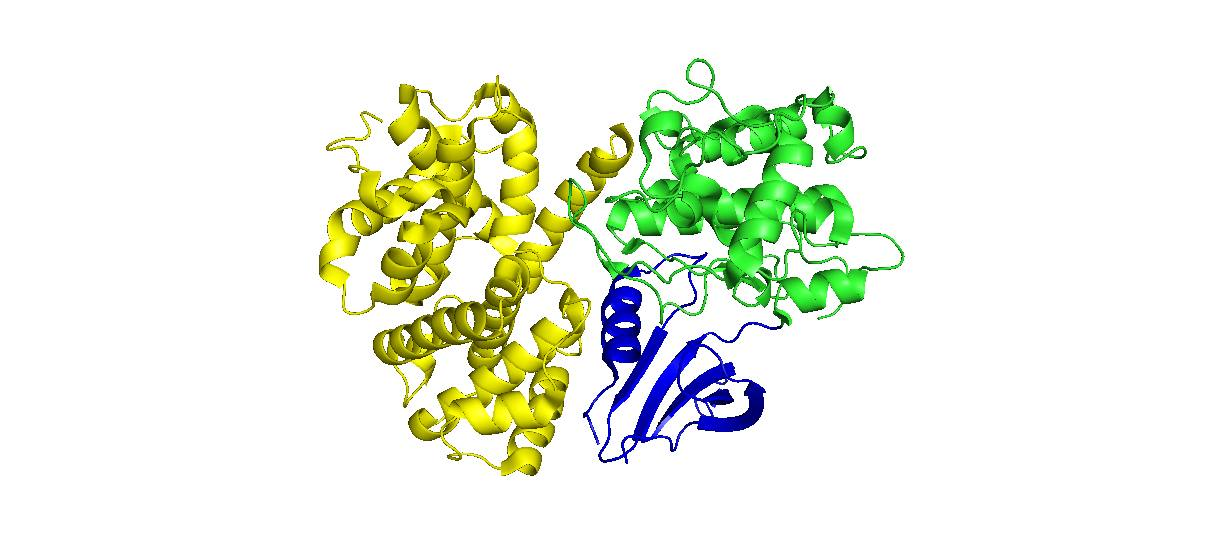
\includegraphics[width=15cm]{./Figures/1a.jpg}

\subsection{Part b}
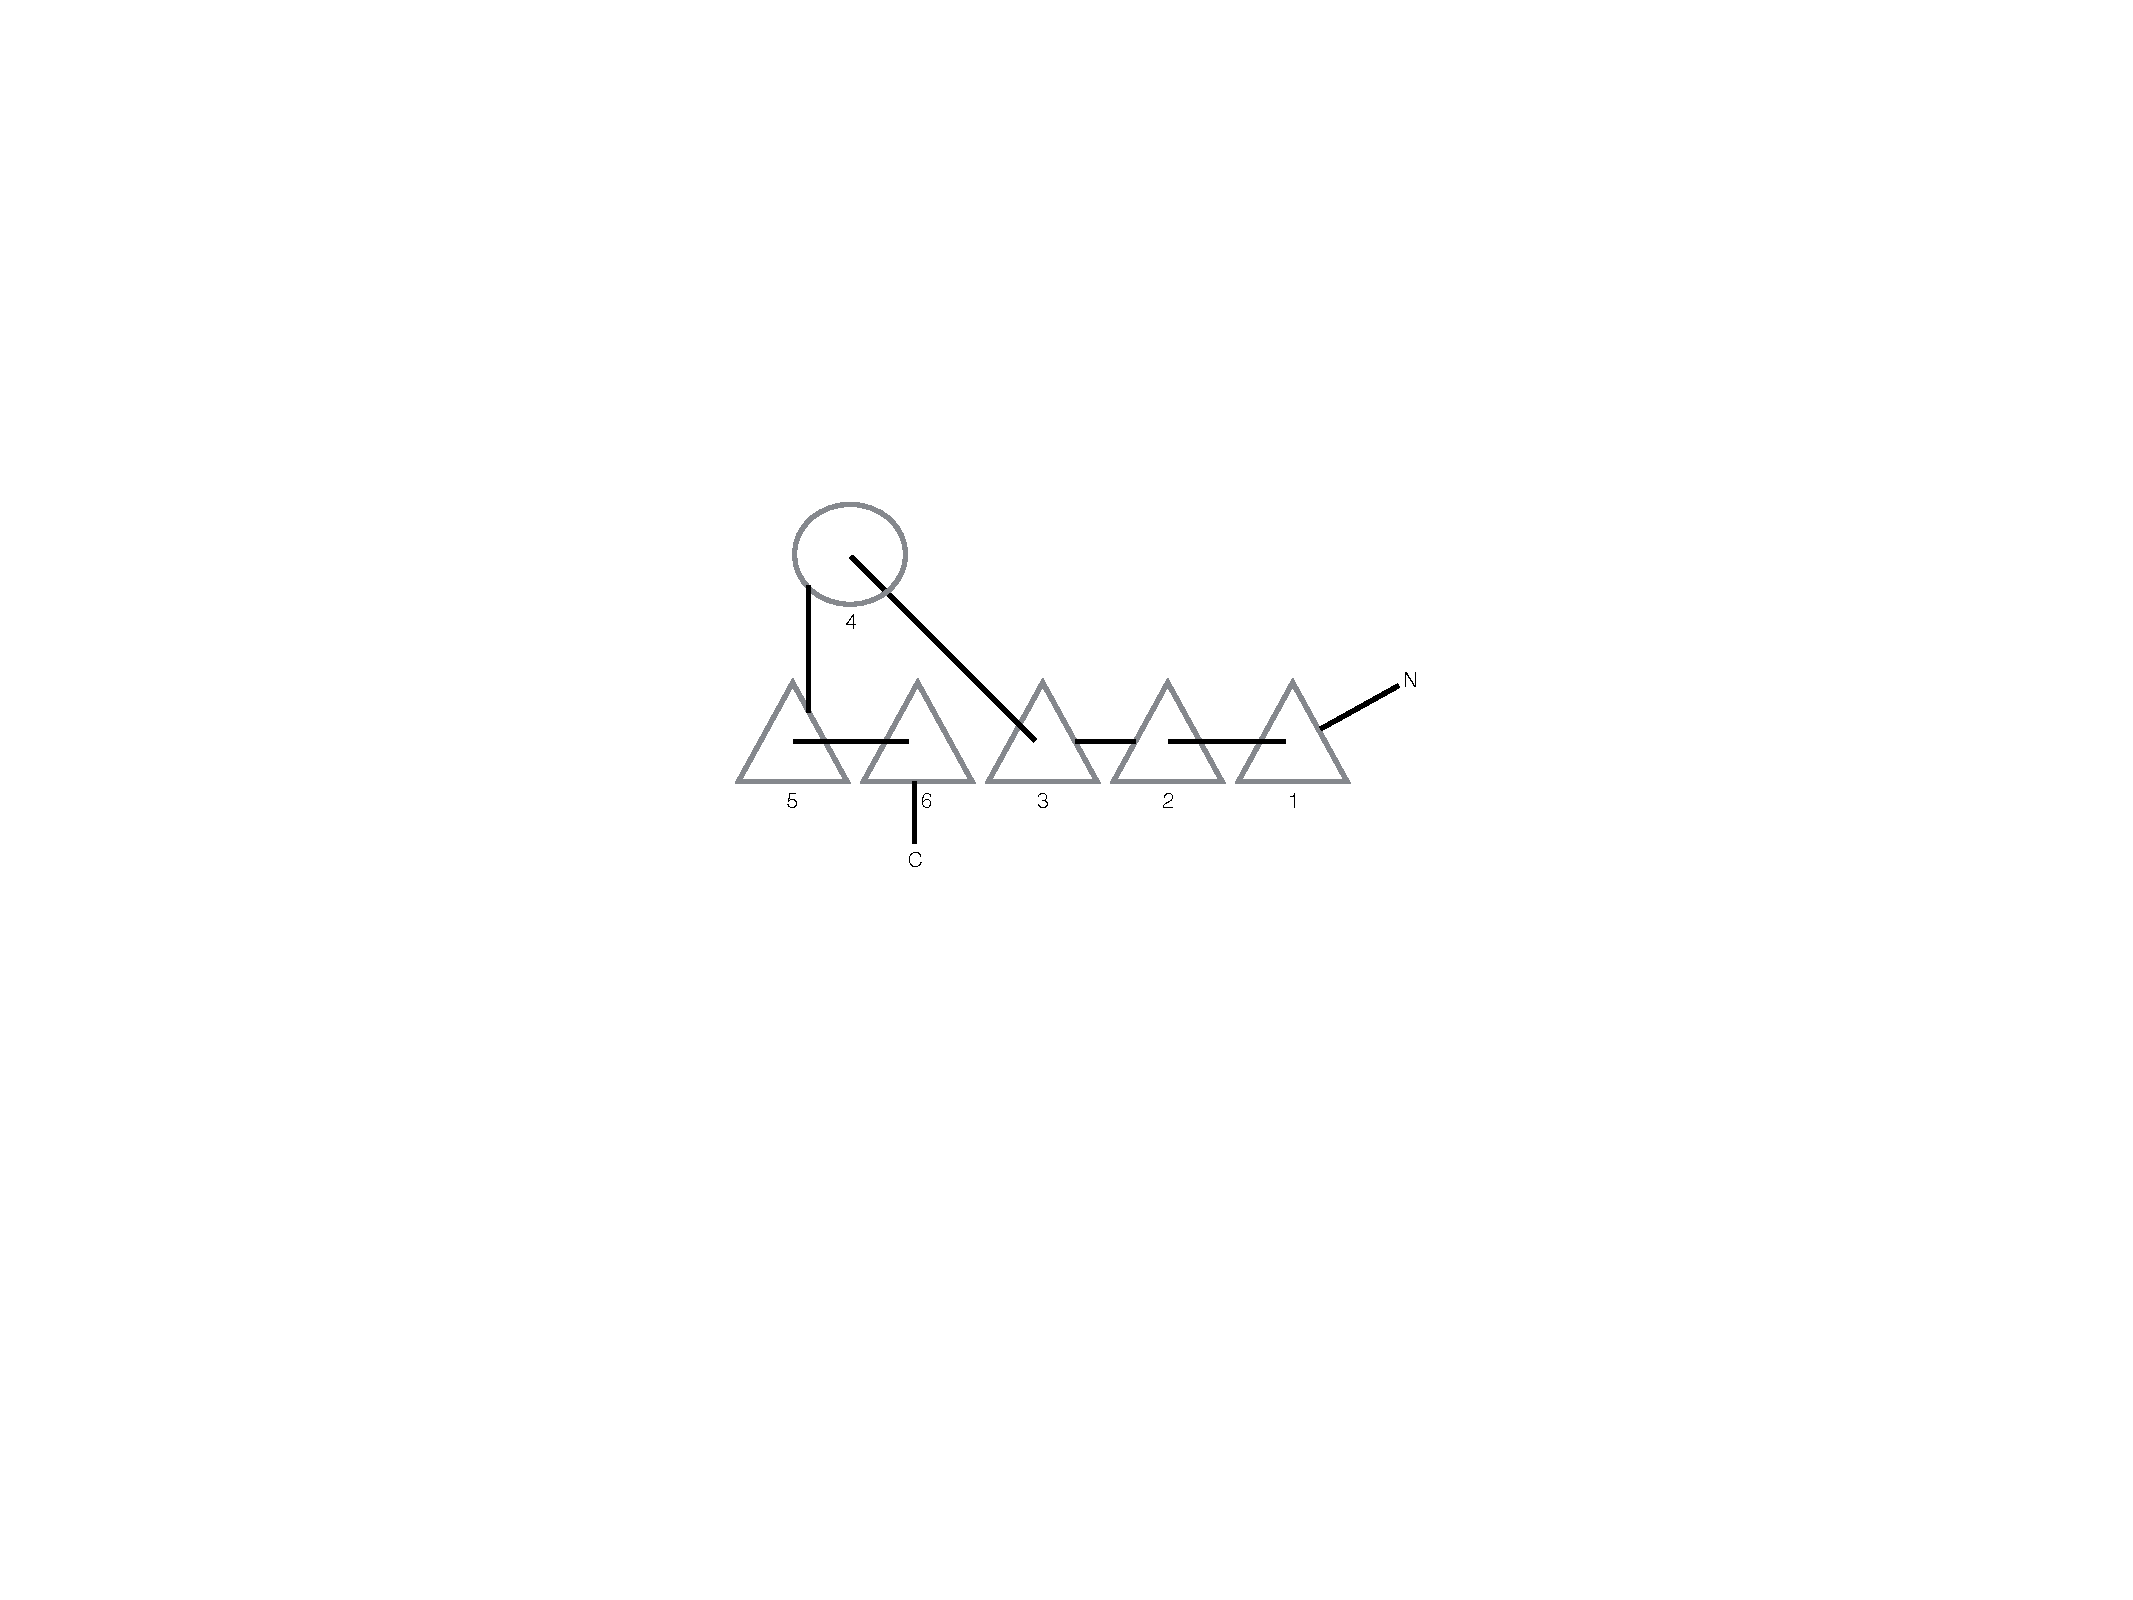
\includegraphics[width=15cm]{./Figures/1b.pdf}

\section{Question 2 - Kinase active/inactive forms}
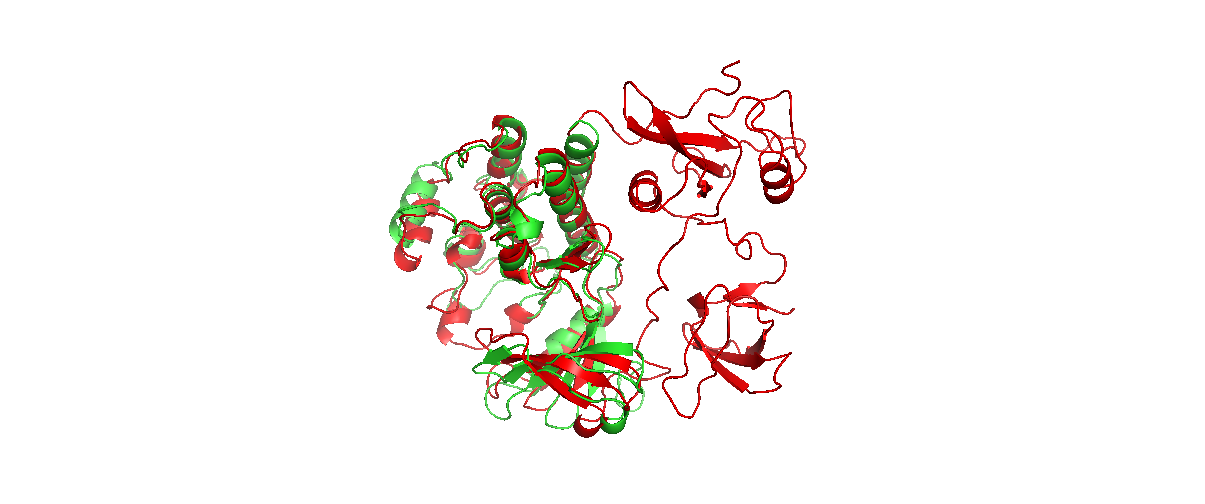
\includegraphics[width=15cm]{./Figures/2a.png}

The role of regulatory domains in the kinases are to induce
conformational changes that switch the kinase from one form (inactive
or active) to the other \cite{ConformationalPlasticityKinases}.

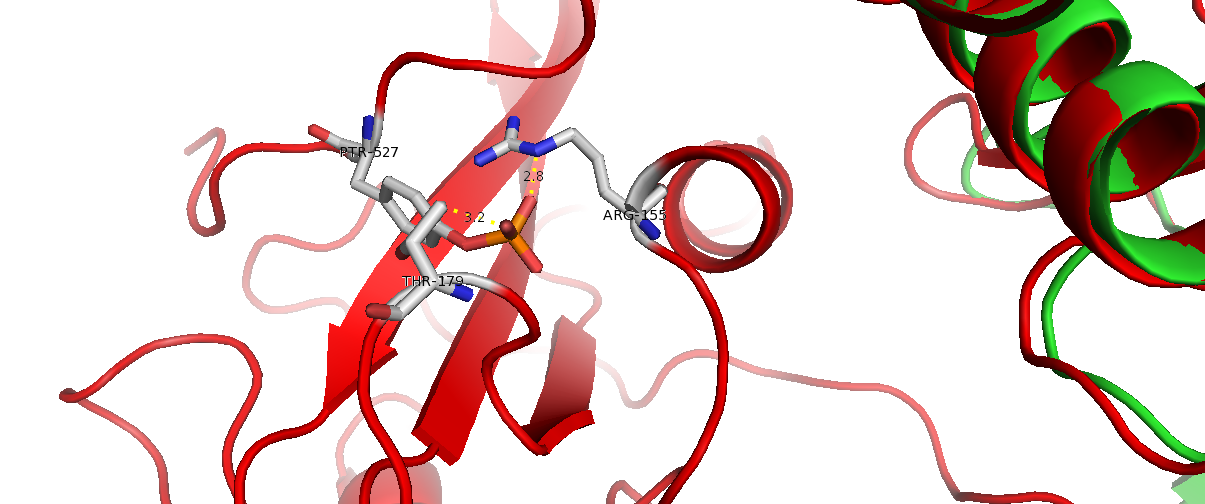
\includegraphics[width=15cm]{./Figures/2b.png}

\section{Question 3 - }

\begin{verbatim}
> table(years)
years
2000 2001 2002 2003 2004 2005 2006 2007 2008 2009 2010 2011 2012 2013 2014 2015 
  41   84   91  131  123  192  224  298  329  309  348  316  426  402  358  102 
> barplot(table(years))
\end{verbatim}

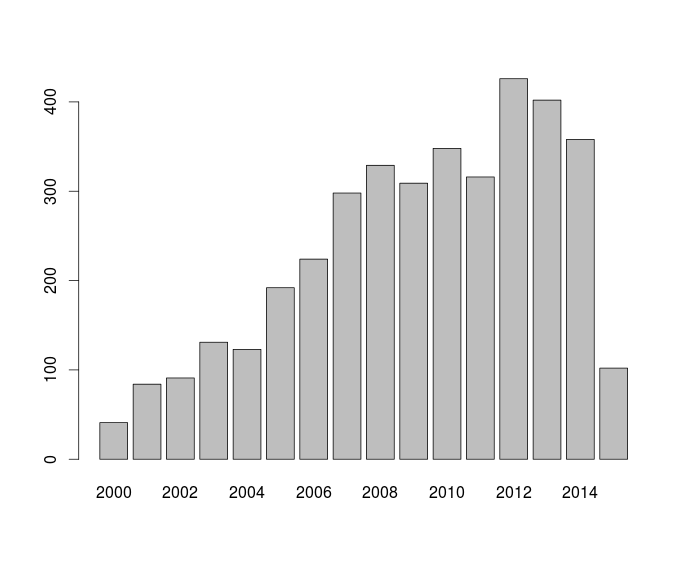
\includegraphics[width=15cm]{./Figures/pdb_kinases_growth.png}
\bibliographystyle{plain}
\bibliography{bib-db}
\end{document}
